\documentclass[10pt,journal,cspaper,compsoc]{IEEEtran}
\usepackage{wrapfig}
 \usepackage{amsmath}
 \usepackage{url}
\usepackage{rotating}
%\usepackage{balance}
\usepackage{color, colortbl}
\usepackage{graphicx}
\usepackage{algorithmicx}
\usepackage{program}
\usepackage{cite}
\usepackage{alltt}
\newcommand{\eq}[1]{Equation~\ref{eq:#1}}
\newcommand{\bi}{\begin{itemize}}
\newcommand{\ei}{\end{itemize}}
\newcommand{\be}{\begin{enumerate}}
\newcommand{\ee}{\end{enumerate}}
\newcommand{\tion}[1]{\textsection\ref{sec:#1}}
\newcommand{\fig}[1]{Figure~\ref{fig:#1}}
\definecolor{lightgray}{gray}{0.975}
\usepackage{fancyvrb}
\usepackage{stfloats}
\usepackage{multirow}
\usepackage{listings}

\usepackage[table]{xcolor}
\definecolor{Gray}{rgb}{0.88,1,1}
\definecolor{Gray}{gray}{0.85}
\definecolor{Blue}{RGB}{0,29,193}

\newcommand{\G}{\cellcolor{green}}
\newcommand{\Y}{\cellcolor{yellow}}
\begin{document}






\begin{figure}
\begin{center}
\small	
\begin{tabular}{|c	|	c	|	c	|	c	|} \hline
Model Name	&	Constrained	&	Runtime	&	Ref	 \\ \hline
BNH-d2-o2	&	Yes	&	0.01	&	\cite{Binh97mobes:a} 	\\	
Viennet3-d2-o3	&	No	&	0.01	&	\cite{viennetmodels} 	\\	
Viennet2-d2-o3	&	No	&	0.01	&	\cite{viennetmodels} 	\\	
Viennet4-d2-o3	&	No	&	0.01	&	\cite{viennetmodels} 	\\	
TwoBarTruss-d3-o2	&	Yes	&	0.01	&	\cite{Chafekar03constrainedmultiobjective} 	\\	
Golinski-d7-o2	&	No	&	0.01	&	\cite{golinskimodel} 	\\	
Water-d3-o5   	&	Yes	&	0.02	&	\cite{watermodel} 	\\	
ZDT6-d10-o2   	&	No	&	0.02	&	\cite{Zitzler2000zdtpaper} 	\\	
DTLZ1-d5-o2   	&	No	&	0.02	&	\cite{dtlz2001a}	\\	
Srinivas-d2-o2	&	Yes	&	0.03	&	\cite{DBLP:journals/ec/SrinivasD94} 	\\	
ZDT4-d10-o2   	&	No	&	0.03	&	\cite{Zitzler2000zdtpaper} 	\\	
DTLZ5-d10-o2  	&	No	&	0.03	&	\cite{dtlz2001a}	\\	
DTLZ2-d10-o2  	&	No	&	0.03	&	\cite{dtlz2001a}	\\	
DTLZ3-d10-o2  	&	No	&	0.03	&	\cite{dtlz2001a}	\\	
DTLZ4-d10-o2  	&	No	&	0.03	&	\cite{dtlz2001a}	\\	
DTLZ2-d10-o4  	&	No	&	0.03	&	\cite{dtlz2001a}	\\	
DTLZ1-d5-o4   	&	No	&	0.04	&	\cite{dtlz2001a}	\\	
DTLZ4-d10-o4  	&	No	&	0.04	&	\cite{dtlz2001a}	\\	
DTLZ3-d10-o4  	&	No	&	0.04	&	\cite{dtlz2001a}	\\	
DTLZ5-d10-o4  	&	No	&	0.04	&	\cite{dtlz2001a}	\\	
ZDT3-d30-o2   	&	No	&	0.05	&	\cite{Zitzler2000zdtpaper} 	\\	
ZDT1-d30-o2   	&	No	&	0.05	&	\cite{Zitzler2000zdtpaper} 	\\	
DTLZ6-d20-o4  	&	No	&	0.05	&	\cite{dtlz2001a}	\\	
ZDT2-d30-o2   	&	No	&	0.06	&	\cite{Zitzler2000zdtpaper} 	\\	
DTLZ6-d20-o2  	&	No	&	0.06	&	\cite{dtlz2001a}	\\	
Osyczka2-d6-o2	&	Yes	&	0.29	&	\cite{osymodel} 	\\	
Tanaka-d2-o2  	&	Yes	&	0.35	&	\cite{537993} 	\\	
xomoos-d27-o4 	&	No	&	0.95	&	\cite{Zitzler2000zdtpaper} 	\\	
xomogr-d27-o4 	&	No	&	0.96	&		\\	
xomofl-d27-o4 	&	No	&	0.96	&		\\	
xomoo2-d27-o4 	&	No	&	0.99	&		\\	
xomoal-d27-o4 	&	No	&	1.01	&		\\	
POM3B-d9-o4   	&	No	&	6.28	&	\cite{port08,me09j}	\\	
POM3A-d9-o4   	&	No	&	218.98	&	\cite{port08,me09j}	\\	
POM3C-d9-o4   	&	No	&	445.03	&	\cite{port08,me09j}	\\	
CDA	&	No	&	8100	&	\cite{Kim2011,Pritchett2011,Feigh2012,Kim2013,Pritchett2013}	\\	\hline
\end{tabular}		
\end{center}
\label{modelruntimes}	
\caption{Model runtimes in milliseconds.  Runtimes obtained from running the standalone model 1000 times with arbitrarily chosen inputs.  The model name is specced in the following format:  \emph{name} - \emph{number of inputs} - \emph{number of objectives}.  For example, ZDT3-d30-o2 means ZDT3 with 30 decision inputs and 2 objective outputs.}
						
\end{figure} 










\begin{figure*}\scriptsize
	\centering
		\begin{tabular}{ | l | c | l@{~} | l@{~} | c@{~} | }
			\hline
			\multicolumn{5}{ | c@{~} | }{Constrained Multi-Objective Functions}\\
			\hline
			Name & n & Objectives & Constraints & Variable Bounds\\\hline \hline	
			
			BNH & 2 & \begin{tabular}{ l@{~} }
				{$ f_1(\vec{x}) = 4*x_1^2 + 4x_2^2 $}\\
				{$ f_2(\vec{x}) = (x_1-5)^2 + (x_2-5)^2 $}\end{tabular} & \begin{tabular}{ l@{~} }
				{$ g_1(\vec{x}) = ( (x_1-5)^2 + 2*x_2^2) <= 25 $}\\
				{$ g_2(\vec{x}) = ( (x_1-8)^8 + (x_2 + 3)^2 ) >=7.7 $}\end{tabular} & \begin{tabular}{ c@{~} }
				{$ 0 <= x_1 <= 5 $}\\
				{$ 0 <= x_2 <= 3$}\\
				\end{tabular}\\ \hline
				
			Osyczka 2 & 6 & \begin{tabular}{ l@{~} }
				{$ A(\vec{x}) = 25 (x_1 - 2)^2 + (x_2 - 2)^2 $}\\
				{$ B(\vec{x}) =  (x_3 - 1)^2*(x_4 - 4)^2 +$}\\
				{$ (x_5 - 2)^2$}\\
				{$ f_1(\vec{x}) =  0 - A - B  $}\\
				{$ f_2(\vec{x}) = x_1^2 + x_2^2 + x_3^2 + $}\\
				{$ x_4^2 + x_5^2 + x_6^2 $} \end{tabular} & \begin{tabular}{ l@{~} }
				{$ g_1(\vec{x}) = x_1 + x_2 - 2 >= 0 $}\\
				{$ g_2(\vec{x}) = 6 - x_1 - x_2 >= 0 $}\\
				{$ g_3(\vec{x}) = 2 - x_2 + x_1 >= 0 $}\\
				{$ g_4(\vec{x}) = 2 - x_1 + 3 x_2 >= 0 $}\\
				{$ g_5(\vec{x}) = 4 - (x_3-3)^2 - x_4 >= 0 $}\\
				{$ g_6(\vec{x}) = (x_5-3)^3 + x_6 - 4 >= 0$}\end{tabular} & \begin{tabular}{ c@{~} }
					{$ 0 <= x_1,x_2,x_6 <= 10 $}\\
					{$ 1 <= x_3,x_4 <= 5 $}\\
					{$ 0 <= x_5 <= 6 $}
				\end{tabular}\\ \hline
				
			Srinivas & 2 & \begin{tabular}{ l@{~} }
				{$ f_1(\vec{x}) = (x_1 - 2)^2 + (x_2-1)^2 + 2 $}\\
				{$ f_2(\vec{x}) = 9x_1 - (x_2 -1)^2 $}\end{tabular} & \begin{tabular}{ l@{~} }
				{$ g_1(\vec{x}) = x_2 + 9x_1 >= 6 $}\\
				{$ g_2(\vec{x}) = -x_2 + 9x_1 >= 1 $}\end{tabular} & {$ -20 <= x <= 20 $}\\\hline

			Tanaka & 2 & \begin{tabular}{ l@{~} }
				{$ f_1(\vec{x}) = x_1 $}\\
				{$ f_2(\vec{x}) = x_2 $}\end{tabular} & \begin{tabular}{ l@{~} }
				{$ A(\vec{x}) = 0.1 \cos{(16\arctan{(\frac{x_1}{x_2})})} $}\\
				{$ g_1(\vec{x}) = 1 - x_1^2 - x_2^2 + A <= 0 $}\\
				{$ g_2(\vec{x}) = (x_1 - 0.5)^2 + $}\\
				{$ (x_2 - 0.5)^2 <= 0.5 $}\end{tabular} & {$ -\pi <= x <= \pi $}\\\hline
				
			Two-bar Truss & 3 & \begin{tabular}{ l@{~} }
				{$ s_1(\vec{x}) = \frac{20*\sqrt{16+x_3^2}}{(x_1*x_3)}    $} \\
				{$ s_2(\vec{x}) = \frac{80*\sqrt{1+x_3^2}}{(x_2*x_3)}    $} \\
				{$ f_1(\vec{x}) = x_1 * \sqrt{16*x_3^2} + x_2*\sqrt{1+x_3^2} $}\\
				{$ f_2(\vec{x}) = max(s_1, s_2) $}\end{tabular} & \begin{tabular}{ l@{~} }
				{$ s_1(\vec{x}) = \frac{20*\sqrt{16+x_3^2}}{(x_1*x_3)}    $} \\
				{$ s_2(\vec{x}) = \frac{80*\sqrt{1+x_3^2}}{(x_2*x_3)}    $} \\
				{$ g_1(\vec{x}) = ( max(s_1, s_2) ) <= 100000 $} \end{tabular} & \begin{tabular}{ c@{~} }
				{$ 0 <= x_1,x_2 <= 0.01 $}\\
				{$ 1 <= x_3 <= 3$}\\
				\end{tabular}\\ \hline

			Water & 3 & \begin{tabular}{ l@{~} }
				{$ f_1(\vec{x}) = 106780.37*(x_2+x_3) + 61704.67$}\\
				{$ f_2(\vec{x}) = 3000*x_1 $}\\
				{$ f_3(\vec{x}) = \frac{(305700*2289*x_2)}{((0.06*2289)**0.65)} $}\\
				{$ E(\vec{x}) = e^{-39.75*x_2+9.9*x_3+2.74} $}\\
				{$ f_4(\vec{x}) = 250*2289*x_2*E(\vec{x}) $}\\
				{$ f_5(\vec{x}) = 25*\frac{1.39}{x_1*x_2+4940*x_3-80} $} \end{tabular} & \begin{tabular}{ l@{~} }
				{$ g_1(\vec{x}) = (   \frac{1 -     0.00139}{x_1*x_2} + 4.94 * x_3 - 0.08  )  $}\\
				{$ g_2(\vec{x}) = (   \frac{1 -     0.000306}{x_1*x_2} + 1.082 * x_3 - 0.0986 ) $}\\
				{$ g_3(\vec{x}) = (   \frac{5000 -     12.307}{x_1*x_2} + 4.9408 * x_3 - 4051.02)  $}\\
				{$ g_4(\vec{x}) = (   \frac{16000 -     2.09}{x_1*x_2} + 804633 * x_3 - 696.71)  $}\\
				{$ g_5(\vec{x}) = (   \frac{10000 -     2.138}{x_1*x_2} + 7883.39 * x_3 - 705.04)  $}\\
				{$ g_6(\vec{x}) = (   \frac{2000 -     0.417}{x_1*x_2} + 1721.26 * x_3 - 136.54) $}\\
				{$ g_7(\vec{x}) = (   \frac{550 -     0.164}{x_1*x_2} + 631.13 * x_3 - 54.48) $}\\
				{$ g_i(\vec{x}) \ge 0 $}\end{tabular} & \begin{tabular}{ c@{~} }
				{$ \frac{1}{100} <= x_1 <= \frac{45}{100} $}\\
				{$ \frac{1}{100} <= x_2,x_3 <= \frac{1}{10}$}\\
				\end{tabular}\\ \hline
		\end{tabular}
		
		\caption[Defining the Constrained Math Models]{Constrained standard mathematical test problems. Note: Objectives to be minimized unless otherwise denoted.}\label{fig:con}
\end{figure*}








\begin{figure*}\small
	\centering
		\begin{tabular}{ | l | c | l@{~} | c@{~} | }
		\hline
		\multicolumn{4}{ | c@{~} | }{Unconstrained Multi-Objective Functions}\\
		\hline
		Name & n & Objectives & Variable Bounds\\\hline\hline
		
		
		
		Golinksi & 7 & \begin{tabular}{ l@{~} }
		{$ r = 0.7854$} \\
		{$ s = 14.933$} \\
		{$ t = 43.0934$} \\
		{$ u = -1.508$} \\
		{$ v = 7.477$} \\
		{$ A(\vec{x}) = r x_1 x_2^2 (\frac{10 x_3^2}{3.0} + s x_3 - t) $}\\
		{$ B(\vec{x}) = u x_1 (x_6^2 + x_7^2)+ v(x_6^3 + x_7^3) + r(x_4*x_6^2 + x_5*x_7^2) $}\\
		{$ aux(\vec{x}) = 745.0 \frac{x_4}{x_2 * x_3} $}\\
		{$ f_1(\vec{x})= A + B $}\\
		{$ f_2(\vec{x})= \frac{\sqrt{aux^2 + 1.69e7}}{0.1 x_6^3} $}
		\end{tabular} & \begin{tabular}{ c@{~} }
		{$ 2.6 <= x_1 <= 3.6 $}\\
		{$ 0.7 <= x_2 <= 0.8 $}\\
		{$ 17.0 <= x_3 <= 28.0 $}\\
		{$ 7.3 <= x_4, x_5 <= 8.3 $}\\
		{$ 2.9 <= x_6 <= 3.9 $}\\
		{$ 5.0 <= x_7 <= 5.5 $} \\
		\end{tabular} \\
		\hline

		Viennet 2 & 2 & \begin{tabular}{ l@{~} }
		{$ f_1(\vec{x})= \frac{(x_1-2)(x_1-2)}{2} + \frac{(x_1+1)(x_1+1)}{13} + 3 $}\\
		{$ f_2(\vec{x})= \frac{(x_1+x_2-3)(x_1+x_2-3)}{36} + \frac{(-x_1+x_2+2)(-x_1+x_2+2)}{8} - 17 $}\\
		{$ f_3(\vec{x})= \frac{(x_1+2x_2-1)(x_1+2x_2-1)}{175} + $} \\ 
		{$ \frac{(2x_2-x_1)(2x_2-x_1)}{17} - 13 $} \\
		\end{tabular} & {$ -4 <= x_i <= 4 $}\\
		\hline
		
		Viennet 3 & 2 & \begin{tabular}{ l@{~} }
		{$ A(\vec{x}) = 3*x_1 - 2*x_2 + 4        $}\\
		{$ B(\vec{x}) = x_1 - x_2 + 1              $}\\
		{$ f_1(\vec{x})=  0.5 * (x_1^2 + x_2^2) + sin(x_1^2 + x_2^2)   $}\\
		{$ f_2(\vec{x})= \frac{A^2  }{ 8 + \frac{B^2}{27} + 15 }      $}\\
		{$ f_3(\vec{x})= \frac{1}{x_1^2 + x_2^2+1} - 1.1 * e^{-(x_1^2) - (x_2^2)}    $} 
		\end{tabular} & {$ -3 <= x_i <= 3 $}\\
		\hline

		Viennet 4 & 2 & \begin{tabular}{ l@{~} }
		{$ f_1(\vec{x})= \frac{(x_1-2)(x_1-2)}{2} + \frac{(x_1+1)(x_1+1)}{13} + 3 $}\\
		{$ f_2(\vec{x})= \frac{(x_1+x_2-3)(x_1+x_2-3)}{175} + \frac{(2*x_2-x_1)*(2*x_2-x_1)}{17} - 13 $}\\
		{$ f_3(\vec{x})= \frac{(3*x_1-2*x_2+4) * ( 3*x_1-2*x_2+4)}{8}   +      $} \\ 
		{$ \frac{(x_1-x_2+1)(x_1-x_2+1)}{27} + 15 $} \\
		\end{tabular} & {$ -4 <= x_i <= 4 $}\\
		\hline

		ZDT1 & 30 & \begin{tabular}{ l@{~} }
		{$ f_1(\vec{x})= x_1 $}\\
		{$ f_2(\vec{x})=  g * (1 - \sqrt{\frac{x_1}{g}})$}\\
		{$ g(\vec{x}) = 1 + \frac{9}{n-1}\sum_{i=2}^{n}(x_i) $}
		\end{tabular} & {$ 0 <= x_i <= 1 $}\\
		\hline

		ZDT2 & 30 & \begin{tabular}{ l@{~} }
		{$ f_1(\vec{x})= x_1 $}\\
		{$ f_2(\vec{x})=  g * (1 - (\frac{x_1}{g})^2)$}\\
		{$ g(\vec{x}) = 1 + \frac{9}{n-1}\sum_{i=2}^{n}(x_i) $}
		\end{tabular} & {$ 0 <= x_i <= 1 $}\\
		\hline
		
		ZDT3 & 30 & \begin{tabular}{ l@{~} }
		{$ f_1(\vec{x})= x_1 $}\\
		{$ f_2(\vec{x})=  g * (1 - \sqrt{(\frac{x_1}{g})} - \frac{x_1}{g} * sin(10*\pi*x_1) )$}\\
		{$ g(\vec{x}) = 1 + \frac{9}{n-1}\sum_{i=2}^{n}(x_i) $}
		\end{tabular} & {$ 0 <= x_i <= 1 $}\\
		\hline
		
		ZDT4 & 10 & \begin{tabular}{ l@{~} }
		{$ f_1(\vec{x})= x_1 $}\\
		{$ f_2(\vec{x})=  g * (1 - \sqrt{(\frac{x_1}{g})} - \frac{x_1}{g} * sin(10*\pi*x_1) )$}\\
		{$ g(\vec{x}) = 1 + 10*(n-1) + \sum_{2}^{n} (x_i^2 - 10*cos(4*\pi*x_i)) $} \\
		\end{tabular} & \begin{tabular}{ c@{~} }
		{$ 0 <= x_1 <= 1 $}\\
		{$ -5 <= x_2,...,x_{10} <= 5$}\\
		\end{tabular}\\
		\hline
		
		ZDT6 & 10 & \begin{tabular}{ l@{~} }
		{$ f_1(\vec{x})=  1 - e^{-4*x_1} * sin(6*\pi*x_1)^6         $}\\
		{$ f_2(\vec{x})=  g * (1  - (\frac{f_1(\vec{x})}{g})^2)  $} \\
		{$ g(\vec{x}) = 1 + 9 * \frac{  \sum_{2}^{n} x_i    }{(n-1)^{0.25}}     $} \\
		\end{tabular} & {$ 0 <= x_i <= 1 $}\\
		\hline


		\end{tabular}
		\caption[Defining the Unconstrained Math Models]{Unconstrained standard mathematical test problems. Note: all objectives
are to be minimized unless otherwise denoted.}
	\label{fig:uncon}

\end{figure*}


\begin{figure*}\small
	\centering
		\begin{tabular}{ | l | c | l@{~} | c@{~} | }
		\hline
		\multicolumn{4}{ | c@{~} | }{DTLZ Family of Models}\\
		\hline
		Name & n & Objectives & Variable Bounds\\\hline\hline
		
		DTLZ1 & n & \begin{tabular}{l@{~} }
		{$ f_1(\vec{x})=  0.5*x_1*x_2*...*x_{M-1}(1+g(x_M))      $}\\
		{$ f_2(\vec{x})=  0.5*x_1*x_2*...*(1 - x_{M-1})(1+g(x_M))      $}\\
		... \\
		{$ f_{M-1}(\vec{x})=  0.5*x_1*(1 - x_2)(1+g(x_M))      $}\\
		{$ f_M(\vec{x})=  0.5*(1 - x_{1})(1+g(x_M))      $}\\
		{$ g(\vec{x}) = 100 * (  |x_M| + \sum (x_i-0.5)^2 - cos(20\pi(x_i-0.5))    )    $} \\
		\end{tabular} & {$ 0 <= x_i <= 1 $}\\
		\hline

		DTLZ2 & n & \begin{tabular}{l@{~} }
		{$ f_1(\vec{x})=  (1+g(X_M)) cos(x_1*\frac{\pi}{2})...cos(x_{M-1}*\frac{\pi}{2})     $}\\
		{$ f_2(\vec{x})=  (1+g(X_M)) cos(x_1*\frac{\pi}{2})...sin(x_{M-1}*\frac{\pi}{2})     $}\\
		... \\
		{$ f_{M}(\vec{x})=  (1+g(X_M)) sin(x_1*\frac{\pi}{2})     $}\\
		{$ g(\vec{x}) = \sum (x_i - 0.5)^2     $} \\
		\end{tabular} & {$ 0 <= x_i <= 1 $}\\
		\hline
		
		DTLZ3 & n & \begin{tabular}{l@{~} }
		{$ f_1(\vec{x})=  (1+g(X_M)) cos(x_1*\frac{\pi}{2})...cos(x_{M-1}*\frac{\pi}{2})     $}\\
		{$ f_2(\vec{x})=  (1+g(X_M)) cos(x_1*\frac{\pi}{2})...sin(x_{M-1}*\frac{\pi}{2})     $}\\
		... \\
		{$ f_{M}(\vec{x})=  (1+g(X_M)) sin(x_1*\frac{\pi}{2})     $}\\
		{$ g(\vec{x}) = 100 * (  |x_M| + \sum (x_i-0.5)^2 - cos(20\pi(x_i-0.5))    )    $} \\
		\end{tabular} & {$ 0 <= x_i <= 1 $}\\
		\hline
		
		DTLZ4 & n & \begin{tabular}{l@{~} }
		{$ f_1(\vec{x})=  (1+g(X_M)) cos(x_1^\alpha*\frac{\pi}{2})...cos(x_{M-1}^\alpha*\frac{\pi}{2})     $}\\
		{$ f_2(\vec{x})=  (1+g(X_M)) cos(x_1^\alpha*\frac{\pi}{2})...sin(x_{M-1}^\alpha*\frac{\pi}{2})     $}\\
		... \\
		{$ f_{M}(\vec{x})=  (1+g(X_M)) sin(x_1^\alpha*\frac{\pi}{2})     $}\\
		{$ g(\vec{x}) = \sum (x_i - 0.5)^2     $} \\
		\end{tabular} & {$ 0 <= x_i <= 1 $}\\
		\hline
		
		DTLZ5 & n & \begin{tabular}{l@{~} }
		{$ f_1(\vec{x})=  (1+g(X_M)) cos(\theta_1*\frac{\pi}{2})...cos(\theta_{M-1}*\frac{\pi}{2})     $}\\
		{$ f_2(\vec{x})=  (1+g(X_M)) cos(\theta_1*\frac{\pi}{2})...sin(\theta_{M-1}*\frac{\pi}{2})     $}\\
		... \\
		{$ f_{M}(\vec{x})=  (1+g(X_M)) sin(\theta_1*\frac{\pi}{2})     $}\\
		{$ \theta_i = \frac{\pi}{4(i+g(r))} (1 + 2g(r)x_i)~for~ i = 2,3,...,(M-1) $}\\
		{$ g(\vec{x}) = \sum (x_i - 0.5)^2     $} \\
		\end{tabular} & {$ 0 <= x_i <= 1 $}\\
		\hline
		
		DTLZ6 & n & \begin{tabular}{l@{~} }
		{$ f_1(\vec{x})=  (1+g(X_M)) cos(\theta_1*\frac{\pi}{2})...cos(\theta_{M-1}*\frac{\pi}{2})     $}\\
		{$ f_2(\vec{x})=  (1+g(X_M)) cos(\theta_1*\frac{\pi}{2})...sin(\theta_{M-1}*\frac{\pi}{2})     $}\\
		... \\
		{$ f_{M}(\vec{x})=  (1+g(X_M)) sin(\theta_1*\frac{\pi}{2})     $}\\
		{$ \theta_i = \frac{\pi}{4(i+g(r))} (1 + 2g(r)x_i)~for~ i = 2,3,...,(M-1) $}\\
		{$ g(\vec{x}) = \sum x_i^{0.1}     $} \\
		\end{tabular} & {$ 0 <= x_i <= 1 $}\\
		\hline

		\end{tabular}
		\caption[Defining the DTLZ Math Models]{DTLZ test problems. Note: all objectives
are to be minimized unless otherwise denoted.}
	\label{dtlzmodels}

\end{figure*}

\begin{figure}
\begin{tabular}{|c|c|c|} \hline
Model & n & M \\ \hline
DTLZ1 & 5   & 2,4  \\
DTLZ2 & 10 & 2,4  \\
DTLZ3 & 10 & 2,4  \\
DTLZ4 & 10 & 2,4  \\
DTLZ5 & 10 & 2,4  \\
DTLZ6 & 20 & 2,4  \\ \hline
\end{tabular}
\caption{Parameter settings for DTLZ models.  n = Number of decisions and M = number of objectives.   Selections for n are made as recommended in \cite{dtlz2001a}.  We run for M = 2 and 4 objectives.}
\end{figure}






\begin{figure}
\scriptsize
\centering
\begin{tabular}{|r|c|c|c|c|} \hline
	&	Model	&	NSGA-II	&	GALE	&	SPEA2	\\ \hline
DTLZ	&	DTLZ1-d5-o2	&	62\%	&	70\%	&	\colorbox{lightgray}{61\%}	\\
Toolkit	&	DTLZ1-d5-o4	&	\colorbox{lightgray}{78\%}	&	83\%	&	\colorbox{lightgray}{78\%}	\\
	&	DTLZ2-d10-o2	&	65\%	&	73\%	&	\colorbox{lightgray}{64\%}	\\
	&	DTLZ2-d10-o4	&	86\%	&	86\%	&	\colorbox{lightgray}{80\%}	\\
	&	DTLZ3-d10-o2	&	65\%	&	73\%	&	\colorbox{lightgray}{64\%}	\\
	&	DTLZ3-d10-o4	&	81\%	&	85\%	&	\colorbox{lightgray}{79\%}	\\
	&	DTLZ4-d10-o2	&	70\%	&	90\%	&	\colorbox{lightgray}{67\%}	\\
	&	DTLZ4-d10-o4	&	93\%	&	92\%	&	\colorbox{lightgray}{90\%}	\\
	&	DTLZ5-d10-o2	&	66\%	&	76\%	&	\colorbox{lightgray}{64\%}	\\
	&	DTLZ5-d10-o4	&	80\%	&	84\%	&	\colorbox{lightgray}{79\%}	\\
	&	DTLZ6-d20-o2	&	67\%	&	71\%	&	\colorbox{lightgray}{67\%}	\\
	&	DTLZ6-d20-o4	&	83\%	&	85\%	&	\colorbox{lightgray}{81\%}	\\ \hline
xomo 	&	xomofl-d27-o4	&	96\%	&	\colorbox{lightgray}{89\%}	&	96\%	\\
models	&	xomogr-d27-o4	&	97\%	&	\colorbox{lightgray}{89\%}	&	97\%	\\
	&	xomoos-d27-o4	&	97\%	&	\colorbox{lightgray}{88\%}	&	97\%	\\
	&	xomoo2-d27-o4	&	96\%	&	\colorbox{lightgray}{89\%}	&	97\%	\\
	&	xomoal-d27-o4	&	96\%	&	\colorbox{lightgray}{87\%}	&	96\%	\\ \hline
POM3 	&	POM3A-d9-o4	&	92\%	&	91\%	&	\colorbox{lightgray}{89\%}	\\
models	&	POM3B-d9-o4	&	92\%	&	\colorbox{lightgray}{90\%}	&	\colorbox{lightgray}{89\%}	\\
	&	POM3C-d9-o4	&	96\%	&	\colorbox{lightgray}{94\%}	&	96\%	\\ \hline
Constrained	&	BNH-d2-o2	&	98\%	&	\colorbox{lightgray}{75\%}	&	97\%	\\
math	&	Osyczka2-d6-o2	&	77\%	&	\colorbox{lightgray}{69\%}	&	78\%	\\
models	&	Srinivas-d2-o2	&	95\%	&	\colorbox{lightgray}{80\%}	&	95\%	\\
	&	Tanaka-d2-o2	&	\colorbox{lightgray}{84\%}	&	85\%	&	85\%	\\
	&	TwoBarTruss-d3-o2	&	95\%	&	\colorbox{lightgray}{78\%}	&	95\%	\\
	&	Water-d3-o5	&	95\%	&	\colorbox{lightgray}{90\%}	&	95\%	\\ \hline
Unconstrained	&	Golinski-d7-o2	&	81\%	&	\colorbox{lightgray}{65\%}	&	81\%	\\
math	&	Viennet2-d2-o3	&	\colorbox{lightgray}{73\%}	&	\colorbox{lightgray}{73\%}	&	\colorbox{lightgray}{73\%}	\\
models	&	Viennet3-d2-o3	&	88\%	&	\colorbox{lightgray}{78\%}	&	88\%	\\
	&	Viennet4-d2-o3	&	90\%	&	\colorbox{lightgray}{77\%}	&	89\%	\\
	&	ZDT1-d30-o2	&	85\%	&	\colorbox{lightgray}{81\%}	&	85\%	\\
	&	ZDT2-d30-o2	&	\colorbox{lightgray}{73\%}	&	\colorbox{lightgray}{72\%}	&	\colorbox{lightgray}{73\%}	\\
	&	ZDT3-d30-o2	&	84\%	&	\colorbox{lightgray}{80\%}	&	85\%	\\
	&	ZDT4-d10-o2	&	\colorbox{lightgray}{68\%}	&	74\%	&	\colorbox{lightgray}{69\%}	\\
	&	ZDT6-d10-o2	&	71\%	&	72\%	&	\colorbox{lightgray}{69\%}	\\ \hline
\end{tabular}
\caption{Median scores comparing final frontier values to
initial populations. Calculated using Equation 1. Lower
scores are better. Gray cells are significantly different
(statistically) and better than the other values in that row.}
\label{whateveryouwannacallme}
\end{figure}



\begin{figure}[!t]
\centering
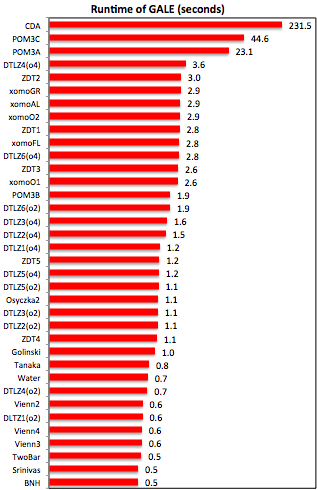
\includegraphics[width=3.0in]{figures/barcharts_runtime_galeAbsolute_v2.png}
\caption{GALE, mean runtime in seconds.}\label{fig:runGale} 
\end{figure}

\begin{figure}[!t]
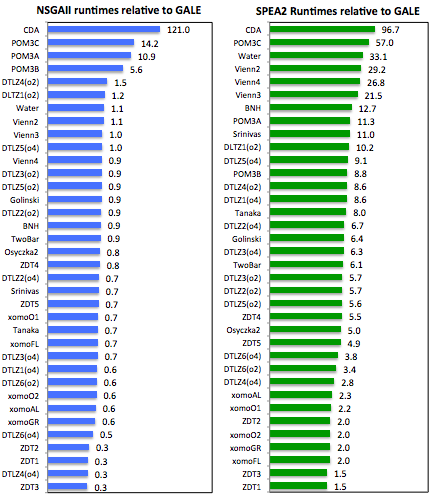
\includegraphics[width=3.5in]{figures/barcharts_runtime_relativeToGale_v2.png}
\caption{NSGA-II, SPEA2, runtimes, relative to GALE (mean values
over all runs) e.g., with SPEA2, ZDT1 ran 1.5 times slower than GALE.}\label{fig:runSpea2} 
\end{figure}

\begin{figure}[!b]
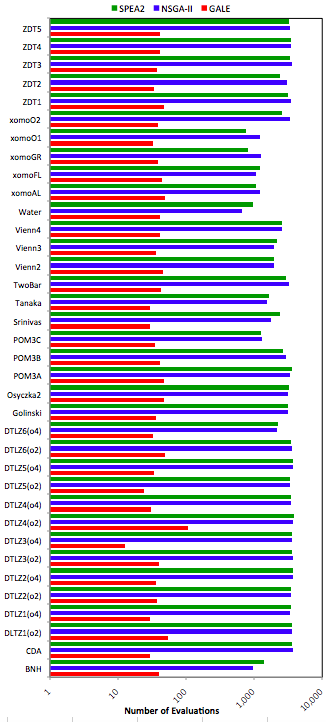
\includegraphics[width=3.5in]{figures/barcharts_numeval_v2.png}
\caption{Number of evaluations (mean values over all runs). Models sorted
by their maximum number of evaluations.}\label{fig:evals} 
\end{figure}




\bibliographystyle{IEEEtran}

\bibliography{references2}


\end{document}
